%%%%%%%%%%%%%%%%%%%%%%%%%%%%%%%%%%%%%%%%%%%%%%%%%%%%%%%%%%%%%%%%%%%%%%
% Lớp 10 | Bất phương trình bậc 2 một ẩn | Phương trình quy về phương trình bậc hai
% Dạng 0D7?3-5: Phương trình khác quy về phương trình bậc 2
% Số câu: 7  (sinh tự động bởi tach_cau.py; từ nay thầy sửa trực tiếp file này)
%%%%%%%%%%%%%%%%%%%%%%%%%%%%%%%%%%%%%%%%%%%%%%%%%%%%%%%%%%%%%%%%%%%%%%

%%%%%%%%%%%%%%%% TRẮC NGHIỆM 4 PHƯƠNG ÁN %%%%%%%%%%%%%%%%

% nguồn: MaHoaNH_TracNghiem_Lop10
\begin{ex}%[0D7N3-5]%[ma:8f91ac01]
	Nghiệm nguyên âm của phương trình $x^2+2x-3=0$  là
	 \choice
		{$x=-3$;  $x=-1$}
		{$x=-3$;  $x=1$}
		{$x=-1$} 
		 {\True $x=-3$}
	\loigiai{Ta có 
		$x^2+2x-3=0 \Leftrightarrow  \hoac{&x=1\\&x=-3.}$\\
		Vậy nghiệm nguyên âm của  phương trình đã cho là $x=-3$.
	} 
\end{ex}

% nguồn: MaHoaNH_TracNghiem_Lop10
\begin{ex}%[0D7H3-5]%[ma:bc1b104b]
	Nghiệm của phương  trình $-2x^{2}+4x-2=0$ là
	\choice 
		 {$x=-1$}
		{$x=-2$} 
		 {$x=2$}
		{\True $x=1$} 
	\loigiai{ 
		Ta có $-2x^{2}+4x-2=0\Leftrightarrow-2(x-1)^{2}=0\Leftrightarrow x=1$. 
	 }
\end{ex}

% nguồn: MaHoaNH_TracNghiem_Lop10
\begin{ex}%[0D7H3-5]%[ma:30984551]
	Cho phương trình $x^{2}-2x+m-5=0$ có hai nghiệm phân biệt $x_{1}$, $x_{2}$ thỏa mãn $x_{1}\cdot x_{2}=-8$. Phương trình có số nghiệm nguyên âm là 
	\choice 
		{$2$} 
		 {$0$}
		{\True $1$} 
		 {$3$}
	 \loigiai{
		Phương trình có hai nghiệm  phân biệt $x_{1}$, $x_{2}$ thỏa mãn $x_{1}\cdot x_{2}=-8$.\\
		 Ta có $\heva{&\Delta'>0\\&x_1\cdot x_{2}=-8}\Leftrightarrow\heva{&-m+6>0\\&m-5=-8}\Leftrightarrow\heva{&m<6\\&m=-3}\Leftrightarrow m=-3$.\\
		Khi đó ta  có phương trình $x^{2}-2x-8=0\Leftrightarrow\hoac{&x=4\\&x=-2.}$\\
		Vậy phương  trình có $1$ nghiệm nguyên âm.
	 }
\end{ex}


%%%%%%%%%%%%%%%% TRẢ LỜI NGẮN %%%%%%%%%%%%%%%%

% nguồn: MaHoaNH_TraLoiNgan_Lop10
\begin{bt}%[0D7H3-5]%[ma:ef07da7f]
	Có tất cả bao nhiêu giá trị nguyên của tham số $m$ để phương trình $mx^2-2(m-1)x+m-3=0$ có  nghiệm duy nhất? \shortans{2}
	\loigiai{ 
		\begin{itemize}
			\item Nếu  $m=0$ thì bất phương trình đã cho trở thành
			\[2x-3=0\Leftrightarrow  x =\dfrac{3}{2}.\]
			Do đó $m=0$, phương trình đã cho có nghiệm duy nhất $x= \dfrac{3}{2}$. 
			 \item Nếu $m \neq 0$ thì $mx^2-2(m-1)x+m-3=0$ là phương trình bậc hai. Phương trình này có nghiệm duy nhất khi
			\[\Delta' =0\Leftrightarrow (m-1)^2-m(m-3)=0\Leftrightarrow m+1=0\Leftrightarrow m=-1 \  \text{(nhận)}.\]
		\end{itemize}
		Vậy với  $m=0$, $m=-1$ thì phương trình đã cho có nghiệm duy nhất.
	} 
\end{bt}

% nguồn: MaHoaNH_TraLoiNgan_Lop10
\begin{bt}%[0D7V3-5]%[ma:7dba8da1]
	Gọi $S$ là tập hợp các giá trị  nguyên của tham số $m\in[3;5]$ để phương trình $(m-2)x^4-2(m+1)x^2-3=0$ có đúng hai nghiệm phân biệt. Tổng các phần tử của tập $S$ bằng bao nhiêu?
	 \shortans{12}
	\loigiai{ 
		Đặt $t=x^2$ ($t\ge0$). 
		Phương trình đã cho  trở thành $(m-2)t^2-2(m+1)t-3=0$ (*)
		\begin{itemize}
			 \item Nếu $m=2$: phương trình đã cho trở thành $-6x^2-3=0\Leftrightarrow x^2=-\dfrac{1}{2}$ (vô nghiệm).
			 \item Nếu $m\ne2$:
			Để phương trình ban đầu có đúng $2$ nghiệm phân biệt thì phương  trình (*) phải có một nghiệm kép dương hoặc có hai nghiệm trái dấu.
			\begin{itemize}
				\item Trường hợp 1: (*) có nghiệm kép  dương khi và chỉ khi\\
				 \[\heva{
				 &\Delta'=0\\
				&\dfrac{m+1}{m-2}>0} 
				 \Leftrightarrow\heva{
				&  m^2+5m-5=0\\
				&  \hoac{&m>2\\&m<-1}
				}\Leftrightarrow  m=\dfrac{-5-3\sqrt{5}}{2}\notin [3;5].\]
				\item Trường hợp 2: (*) có  hai nghiệm trái dấu $\Leftrightarrow -3(m-2)<0\Leftrightarrow m>2$.
			\end{itemize}
			Vậy $S=\{3;4;5\}$ nên tổng  các phần tử của tập $S$ là $12$.
		\end{itemize}
	} 
\end{bt}

% nguồn: MaHoaNH_TraLoiNgan_Lop10
\begin{bt}%[0D7C3-5]%[ma:db8c08b3]
	Có tất  cả bao nhiêu số tự nhiên $m$ sao cho phương trình $\left|x^2-4x+m-1\right|=2x+2$ có đúng hai nghiệm cùng dương?
	 \shortans{8}
	\loigiai{ 
		Do  $x\geq0$ nên $x+2\geq0$.\\
		Khi đó ta có 
		\allowdisplaybreaks 
		\begin{eqnarray*}
			 &&\left|x^2-4x+m-1\right|=2x+2\\
			&\Leftrightarrow&\hoac{&x^2-4x+m-1=2x+2\\&x^2-4x+m-1=-2x-2}\\ 
			 &\Leftrightarrow&\hoac{&x^2-6x+m-3=0\\&x^2-2x+m+1=0}\\
			 &\Leftrightarrow&\hoac{&-x^2+6x+3=m&(1)\\&-x^2+2x-1=m&(2)}
		\end{eqnarray*}
		 \textbf{Trường hợp 1:}\\
		Đặt $f(x)=-x^2+6x+3$ là hàm  số bậc hai có tọa độ đỉnh là $\left(-\dfrac{b}{2a};-\dfrac{\Delta}{4a}\right)=\left(3;12\right)$.\\
		 Bảng biến thiên
		\begin{center}
			\begin{tikzpicture}[scale=1]
					 \tkzTabInit[nocadre=false,lgt=1.5,espcl=5,deltacl=0.6]{$x$/0.7,$f (x)$/2}
						{$0$,$3$,$+\infty$} 
					 \tkzTabVar{-/$3$,+/$12$,-/$-\infty$}
				\end{tikzpicture}
		\end{center}
		Ta thấy  $m\in(3;12)\Rightarrow(1)$ có hai nghiệm dương phân biệt, $m\leq3\Rightarrow(1)$ có một nghiệm dương.\\
		 \textbf{Trường hợp 2:}\\
		 Đặt $f(x)=-x^2+2x-1$ là hàm số bậc hai có tọa độ đỉnh là $\left(-\dfrac{b}{2a};-\dfrac{\Delta}{4a}\right)=\left(1;0\right)$.\\
		Bảng biến  thiên
		\begin{center}
			\begin{tikzpicture}[scale=1]
					\tkzTabInit[nocadre=false,lgt=1.5,espcl=5,deltacl=0.6]{$x$/0.7,$f  (x)$/2}
						{$0$,$1$,$+\infty$} 
					 \tkzTabVar{-/$-1$,+/$0$,-/$-\infty$}
				\end{tikzpicture}
		\end{center}
		Ta thấy $m\in(-1;0)\Rightarrow(2)$ có hai nghiệm dương phân biệt,  $m\leq -1\Rightarrow(2)$ có một nghiệm dương.\\
		Số nghiệm của phương trình ban đầu là kết hợp nghiệm của hai trường  hợp trên.\\
		Khi $3<m<12$ thì $(1)$ có hai nghiệm phân biệt dương, $(2)$ vô nghiệm (thỏa  mãn).\\
		 Suy ra $m\in\{4;5;\ldots11\}\Rightarrow$ có $11-4+1=8$ giá trị $m$ nguyên dương thỏa yêu cầu.\\
		Khi $-1\leq m$ thì $(1)$ có một nghiệm phân biệt dương, $(1)$ có một nghiệm. Lúc đó phương trình ban đầu cũng có hai nghiệm phân biệt dương nhưng $m<0$ không thỏa  $m$ dương (loại).
	} 
\end{bt}


%%%%%%%%%%%%%%%% TỰ LUẬN %%%%%%%%%%%%%%%%

% nguồn: MaHoaNH_TuLuan_Lop10
\begin{bt}%[0D7H3-5]%[ma:445565f5]
	Tìm tập nghiệm của phương trình sau: $\sqrt{x^2-3x+3} + \sqrt{x^2-3x+6}  = 3$.
	\loigiai{ 
		Đặt $t = \sqrt{x^2-3x+3}$ ($t \ge 0$), suy ra $t^2 =  x^2 - 3x + 3 \Rightarrow t^2 - 3 = x^2 - 3x$.\\
		Phương trình  trở thành
		\begin{eqnarray*}
			& & t + \sqrt{(t^2 - 3) + 6}  = 3\\
			&\Leftrightarrow & \sqrt{t^2 + 3} = 3 -  t\\
			&\Leftrightarrow & \begin{cases} 3 - t \ge 0 \\ t^2 + 3 = 9 - 6t + t^2
		\end{cases}\\
		&\Leftrightarrow &\heva{&t \le 3 \\& t  = 1} \Rightarrow t = 1
	\end{eqnarray*}
	Với $t =  1$, ta có
	\begin{eqnarray*}
		& & \sqrt{x^2 - 3x + 3} =  1\\
		&\Leftrightarrow & x^2 -  3x + 3 = 1\\
		 &\Leftrightarrow & x^2 - 3x + 2 = 0\\
		&\Leftrightarrow &x = 1 \vee x  = 2
	\end{eqnarray*}
	Vậy tập nghiệm của phương trình  là $S = \{1; 2\}$.
} 
\end{bt}
